\setcounter{chapter}{8}
\chapter{Асинхронно-событийное программирование}
\section{Работа операционной системы}
\subsection{Параллелизм и псевдопараллелизм}%4 0:49

\textbf{Процесс} --- код программы в виде последовательности команд, который загружен в память, имеет регистры, прерывания и стек, и исполняется на процессоре. Если единственный процесс исполняется на единственном процессоре, он занимает процессор эксклюзивно. Когда не было многоядерных систем, операционные системы для достижения многозадачности использовали псевдопараллелизм. \textbf{Псевдопараллелизм} --- исполнение нескольких процессов на одном физическом процессоре в условиях разделения времени.

Чтобы обеспечить разделение времени, вводится понятие состояния процесса.
%\begin{figure}[H]\end{figure}
Процесс может исполняться, находиться в готовности (пока исполняется другой процесс) или в состоянии блокировки (ожидать выполнения какого-либо вызова). Управляет состояниями процессов операционная система. Операционную систему можно мыслить как главную программу, которая управляет другими исполняемыми программами. Когда в системе исполняются более одного процесса постоянно происходит так называемое переключение контекста, в ходе которого операционной системе необходимо:
\begin{enumerate}[nosep]
  \item обработать прерывание таймера
  \item сохранить регистры
  \item сохранить стек
  \item выбрать новый процесс
  \item загрузить регистры
  \item загрузить стек
\end{enumerate}
В ядре Linux можно задать частоту таймера, которая раньше по умолчанию для серверных систем была равна 100HZ. Это приводило к тому, что в рамках одной системы может быть не более 100 переключений контекста в секунду. Грубо говоря 100 процессов еще будут работать нормально, но если процессов будет 101, какому-то из них постоянно не будет хватать процессорного времени. Разумеется, современные системы организованы более продуманно. Тем не менее, в большинстве случаев, переключение контекстов --- затратная операция.

\subsection{Системные вызовы ввода-вывода}
Загрузка процессора постоянно на 100\% невозможна, так как все процессы большую часть времени ожидают окончание операции ввода-вывода и в это время не исполняются. Если $p$~--- часть времени ожидания ввода вывода, $n$~--- степень многозадачности, то загрузка ЦП будет:
\[ \mathrm{CPU} = (1 - p^n)\cdot 100\%. \]
\begin{figure}[H]\centering
  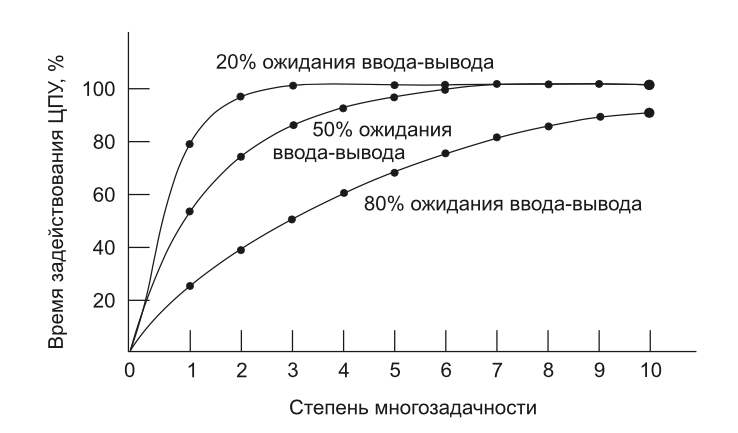
\includegraphics[width=14cm]{lectures/L9/power-of.png}
  \caption{Зависимость загрузки ЦП от степени многозадачности.}
\end{figure}
Процессы ожидают, в основном, выполнение системных вызовов, которые по сути являются запросами к ОС на выполнение привилегированных операций. Это необходимо, так как ОС исполняется в привилегированном режиме с доступом ко всему оборудованию, в отличие от пользовательских процессов. Выполнение системного вызова происходит следующим образом:
\begin{enumerate}[nosep]
  \item Прерывание
  \item передача управления ос
  \item проверка привилегий
  \item работа с оборудованием
  \item загрузка данных для программы
  \item возврат управления
\end{enumerate}
Системный вызов ввода-вывода несколько сложнее. Например, запись на жесткий диск с помощью Си-функции \verb|write| происходит следующим образом:
\begin{enumerate}[nosep]
  \item Прерывание
  \item передача управления ос
  \item проверка привилегий
  \item работа с оборудованием
  \item установка обработчика прерывания
  \item context switch
  \item ...
  \item context switch
  \item загрузка данных для программы
  \item возврат управления исходному процессу
\end{enumerate}
После того, как работа с оборудованием завершена, происходит context switch и исполняется другой процесс до тех пор, пока не сработает прерывание контроллера диска. После этого управление возвращается к исходному процессу.

Простой tcp-сервер приблизительно выглядит так:
\begin{minted}{perl}
while (1) {
    accept
    fork
        read
        write
        read
        write
        ...
        close
        exit
}
\end{minted}
Производительность современных процессоров настолько велика, что время ожидания выполнения read и write значительно превосходит время, затраченное на выполнение остальных операций. Казалось бы, если ожидание ввода-вывода составляет 99.99\% времени исполнения каждого процесса, то можно было бы запустить около 10000 процессов и загрузка ЦП составила бы около 63\%. На практике это не так и эта проблема носит название <<проблема 10000 соединений>>: главным препятствием становится ограничение на размер оперативной памяти, а также необходимость огромного числа переключений контекста.

\subsection{Блокирующие и неблокирующие операции ввода-вывода}
Обычная блокирующая операция ввода-вывода выглядит так:
\begin{minted}{perl}
read(...) -> SUCCESS
read(...) -> FATAL ERROR
\end{minted}
В результате выполнения операции либо успех, либо неудача.

Неблокирующие операции ввода вывода несколько отличаются:
\begin{minted}{perl}
read(...) -> SUCCESS
read(...) -> TEMPORARY ERROR
read(...) -> FATAL ERROR
\end{minted}
Может либо сразу возвращен успех или неудача, а также может быть возращена временная ошибка. Временная ошибка значит, что данная операция временно невозможна.

Это дает возможность писать приложение, работающее на одном ядре, в один процесс, но которое сможет обрабатывать множество различных дескрипторов:
\begin{minted}{perl}
while (1) {
    for my $fh (@fds) {
        my $res = read($fh, ...);
        if ($res) {
            # do work
        }
        elsif ($! ~~ FATAL_ERROR) { # pseudocode
            # close fh, remove from @fds
        }
        else {
            # wait
        }
    }
}
\end{minted}
Это бесконечный цикл, а значит будет расходовать все процессорное время, но это уже некоторое решение, позволяющее обрабатывать большое количество дескрипторов в одном процессе. Соответственно, чтобы избежать загрузки ЦПУ из-за неэффективности цикла был придуман вызов \textbf{select}, который доступен практически в любом языке программирования с доступом к ОС. В вызове select передается вектор сокетов для чтения, вектор дескрипторов для записи и вектор дескрипторов для отслеживания ошибок:
\begin{minted}{perl}
($found,$timeleft) =
    select(
        $readable, # vec
        $writable, # vec
        $errors,   # vec
        $timeout   # in fractional seconds
    )
\end{minted}
Функция vec проставляет конкретный бит или набор бит в строке:
\begin{minted}{perl}
vec($readable, fileno(STDIN),  1) = 1;
vec($readable, fileno(STDOUT), 1) = 1;
vec($readable, fileno(STDERR), 1) = 1;

say unpack "B*", $readable; # 00000111
\end{minted}
Функция \verb|select| возвращает количество готовых дескрипторов и какое время осталось до окончания таймаута.

\section{Интерфейс IO::Select}
Существует интерфейс \verb|IO::Select|, который позволяет удобно работать все с той же функцией \verb|select|:
\begin{minted}{perl}
use IO::Select;

$s = IO::Select->new();

$s->add(\*STDIN);
$s->add($fd);

@ready = $s->can_read($timeout);
\end{minted}
В данном коде показано, как добавлять и удалять дескриптор. На данном этапе уже можно написать нечто более сложное, так как уже можно принимать соединения, добавлять их в select, смотреть, какие готовы, и обрабатывать их. Но существует проблема, что reed, write и т.д являются блокирующими вызовами.

В POSIX был введён флаг \verb|O_NONBLOCK| для \textbf{Fcntl}:
\begin{minted}{perl}
use Fcntl qw(F_GETFL F_SETFL O_NONBLOCK);

$flags = fcntl($fd, F_GETFL, 0)
    or die "Can't get flags for the socket: $!\n";

$flags = fcntl($fd, F_SETFL, $flags | O_NONBLOCK)
    or die "Can't set flags for the socket: $!\n";
\end{minted}
Если применить его на дескриптор, то на этом дескрипторе будет запрещено выполнять блокирующие операции. Любое обращение на этом дескрипторе не заблокируются, а выстовят одну из следующих ошибок:
\begin{itemize}
  \item \textbf{EAGAIN} --- <<попробуй позже>>, штатный ответ, что сокет не готов к запрошенной операции. Это значит, что данный сокет нужно положить в  select на готовность к этой операции.
  \item \textbf{EWOULDBLOCK} --- то же, что и EAGAIN (в большинстве ОС). EWOULDBLOCK значит, что <<если это сделать, то сокет бы заблокировался>>.
  \item \textbf{EINTR} --- <<выполнение системного вызова было прервано прерыванием>>. В этом случае вызов нужно просто повторить.
\end{itemize}
Например, чтение из сокета принимает вид:
\begin{minted}{perl}
use Errno qw(EAGAIN EINTR EWOULDBLOCK);

my $read = sysread($fd, my $buf, SOMELENGTH);

if ($read) { # read >= 0
    # work with data in buf
}
elsif (defined $read) { # read == 0
    # socket was closed
}
elsif ( $! ~~ [ EAGAIN, EINTR, EWOULDBLOCK ] ) {
    # socket not ready for reading
}
else {
    # socket was closed with error $!
}
\end{minted}
Следует отметить, что при блокирующих вызовах sysread считывает нужную длину строки, а при неблокирующих --- считывает столько, сколько может считать.

\section{Цикл событий}
Можно использовать упрощенную схему (описана не очень правильно, но для примера подойдет):
\begin{minted}{perl}
use IO::Select; my $s = IO::Select->new();

my $timeout = 1;
# prepare program...

while () {
    my @ready = $s->can_read($timeout);
    for (@ready) { # do reads }

    my @ready = $s->can_write($timeout);
    for (@ready) { # do writes }
}
\end{minted}
В программе создается один глобальный Select и задается timeout для цикла. После этого запускается так называемый \verb|Event loop|, внутри которого происходят операции ввода-вывода. Создание сокетов происходит на этапе подготовки. Например, в случае сервера нужно создать слушающий сокет и записать его в select.

Удобнее пользоваться замыканиями:
\begin{minted}{perl}
{
    my `$var` = rand();

    my $sub = sub {
        print `$var`;
    }
}
\end{minted}
Замыкания предоставляют возможность сослаться из области видимости некой функции, расположенной ниже, на переменную, объявленную в scope выше:
\begin{minted}{perl}
{
    my `$var` = rand(); # .42;
    my $sub = sub {
        # my $var = .42;
        print `$var`;
    }
}
\end{minted}
Можно сделать генератор функций:
\begin{minted}{perl}
sub decorator {
    my $decor = shift;
    return sub {
        return $decor."@_".$decor;
    }
}

my $dq = decorator "'";
my $dd = decorator '"';
my $ds = decorator '/';

say $dq->('test');  # 'test'
say $dd->('test');  # "test"
say $ds->('test');  # /test/
\end{minted}
В данном примере возвращается функция, которая замыкает переданный при генерации параметр, и добавляет к своему строковому аргументу его слева и справа.

Ещё один пример, набор функций, в которых прибавляется значение к своему аргументу:
\begin{minted}{perl}
my @subs;

for my $var (1..10) {
    my $sub = sub {
        return $var + $_[0];
    };
    push @subs, $sub;
}

for my $sub (@subs) {
    say $sub->(2);
}
# 3 4 5 6 7 8 9 10 11 12

for my $sub (@subs) {
    say $sub->(10);
}
# 11 12 13 14 15 16 17 18 19 20
\end{minted}

Это позволяет замыкать дескриптор внутри некоторой функции (называется callback):
\begin{minted}{perl}
my $fd = socket...
wait_socket_readable($fd, sub {
    read($fd, ...)
})

# ...

our %waiters;
sub wait_socket_readable {
    my ($fd,$cb) = @_;
    $select->add($fd);
    push @{ $waiters{$fd} }, $cb;
}
# Event loop:
while () {
    # ...
    for my $fd (@ready) {
        for my $cb ( @{ $waiters{$fd} } ) {
            $cb->();
        }
    }
}
\end{minted}
Так как эта функция сразу не готова вернуть результат, она передается функции \verb|wait_socket_readable|, которая добавляет сокет в \verb|select|, а ссылку на функцию в специальный хеш. После этого внутри event loop для всех готовых дескрипторов вызываются функции, которые ждали их готовности.

Это позволяет нам писать последовательные цепочки кода:
\begin{minted}{perl}
my $fd = socket...

wait_socket_readable($fd, sub {
    sysread($fd, ...);

    wait_socket_writable($fd, sub {
        syswrite($fd, ...);

        wait_socket_readable($fd, sub {
            sysread($fd, ...);

            # ...
        });
    });
});

# ...
        my @wait = @{ $waiters{$fd} };
        @{ $waiters{$fd} } = ();
        for my $cb ( @wait ) {
\end{minted}

Также может потребоваться ограничить время ожидания сокета, например секундой. Для этого можно сделать функцию, которая представляет собой таймер:
\begin{minted}{perl}
wait_timeout 1, sub { ... };

our @deadlines;
sub wait_timeout {
    my ($t,$cb) = @_;
    my $deadline = time + $t;
    @deadlines =
        sort { $a->[0] <=> $b->[0] }
        @deadlines, [ $deadline, $cb ];
}

# Event loop:
while () {
    #...
    while ($deadlines[0][0] <= time) {
        my $next = shift(@deadlines);
        my $cb = $next->[1];
        $cb->();
    }
}
\end{minted}
В event loop, помимо работы с сокетами, содержится цикл по deadline.

В этом примере применен довольно примитивный подход (для примера): здесь просто применен sort на каждую операцию, что плохо, так как есть гораздо более адекватные алгоритмы вставки элемента в массив.

Здесь есть одна опасность. Пусть дан следующий код:
\begin{minted}{perl}
wait_timeout 1, sub {
    wait_timeout 0, sub {
        wait_timeout 0, sub {
            wait_timeout 0, sub {
                wait_timeout 0, sub {
                    wait_timeout 0, sub {
                        wait_timeout 0, sub {
                            ...
                        };
                    };
                };
            };
        };
    };
};
\end{minted}
Его можно свернуть до такого кода:
\begin{minted}{perl}
wait_timeout 1, sub {
    my $sub; $sub = sub {
        wait_timeout 0, $sub;
    }; $sub->();
};
\end{minted}
В event loop вызывается callback для первого элемента массива deadlines и этот элемент удаляется из массива:
\begin{minted}{perl}
my $deadline = time + $t;
unshift @deadlines, [$deadline, $cb];
# ...
    while ($deadlines[0][0] <= time) {
        my $next = shift(@deadlines);
        my $cb = $next->[1];
        $cb->();
    }
\end{minted}
Но при исполнении callback'а в массив deadlines добавляется очередной элемент. Получается зацикливание. Это нехорошо, таймеры не должны себя так вести.

Поэтому необходимо сделать следующее:
\begin{itemize}
  \item Необходимо зафиксировать время (сохранить в переменную \verb|$now|) и пока идет выполнение цикла эта переменная не должна меняться.
  \item Внутри цикла все расчеты, сравнения и так далее должны выполняться относительно этого фиксированного времени.
  \item Чтобы избежать зацикливания, event loop необходимо переписать: сначала извлечь все таймеры, для которых нужно выполнить callback, а затем выполнить соответствующие callback'и. В ходе выполнения callback'ов массив \verb|@deadlines| может пополниться, но это уже не будет влиять на исполнение цикла.
\end{itemize}
Получается следующий код:
\begin{minted}{perl}
our `$now`;
our @deadlines;

sub wait_timeout {
    my ($t,$cb) = @_;
    my $deadline = `$now` + $t;
    @deadlines =
        sort { $a->[0] <=> $b->[0] }
        @deadlines, [ $deadline, $cb ];
}
# Event loop:
while () {
    `$now` = time;
    #...
    my @exec;
    push @exec, shift @deadlines
        while ($deadlines[0][0] <= `$now`);
    for my $dl (@exec) {
        $dl->[1]->();
    }
}
\end{minted}

\section{Обобщенный интерфейс}
Предыдущие рассуждения приводят к некому обобщённому интерфейсу:
\begin{minted}{perl}
io( $fd, READ | WRITE, $cb);
timer( $timeout, $cb );
runloop();
\end{minted}
Есть функция io, которая принимает дескриптор, требуемое действие и callback. Также есть возможность задать таймер на какое-то время. Функция runloop(); вызывается один раз и запускает основной цикл.

Если до запуска основного цикла не были установлены никакие ожидания ввода/вывода и не были установлены таймеры, этот цикл представляет собой бесконечный цикл, в который никак невозможно войти. Поэтому во многих реализациях event loop он реализован таким образом, что в такого рода ситуации просто выходит.

Для perl была написана библиотека AnyEvent, которая представляет такую абстракцию (обобщенный интерфейс) поверх совершенно различных реализаций событийных циклов. Здесь стоит отметить, что одновременно использовать два событийных цикла нельзя: функция запуска цикла является блокирующей. AnyEvent позволяет писать программу, не задумываясь о реализации конкретно используемого событийного цикла, используя следующий интерфейс:
\begin{minted}{perl}
AE::io( $fd, $flag, $cb );
AE::timer( $after, $interval, $cb );
AE::signal( $signame, $cb );
AE::idle( $cb );
AE::now();
\end{minted}
Часто используется событийный цикл AnyEvent::loop, написанный на чистом perl с использованием select.

\section{Модуль AnyEvent}
\subsection{Интерфейс AE::io}%38 31:32
В AE::io есть два интерфейса:
\begin{itemize}
\item \textbf{объектный}: вызывается метод io объекта AnyEvent:
\begin{minted}{perl}
AnyEvent->io( fd=>\*STDIN, poll=>'r',
    cb => sub {
        my $line = <STDIN>;
        AnyEvent->io( fd=>\*STDOUT, poll=>'w',
            cb => sub {
                print $line;
            }
        );
    }
);
\end{minted}
\item \textbf{сокращённый}: вызывается функция, которой передаются 3 аргумента:
\begin{minted}{perl}
AE::io \*STDIN, 0, sub {
    # stdin is readable;
    my $line = <STDIN>;
    AE::io \*STDOUT, 1, sub {
        # stdout is writable
        print $line;
    };
};
\end{minted}
\end{itemize}
Сокращенный интерфейс чуть-чуть быстрее и компактнее выглядит, поэтому примеры будут приведены именно используя сокращенный интерфейс.
% TODO Про использование  функциями класса SYS

В приведенном примере есть одна проблема: блок, который выполняется, если STDOUT готов к записи будет выполняться бесконечно. Чтобы решить эту проблему можно использовать модуль Guard:
\begin{minted}{perl}
my $guard = guard { # same as guard(sub { ... })
    say '$guard was unrefed';
};
say "Before...";
undef $guard;
say "After";
\end{minted}
Функция guard принимает в качестве параметра блок кода и возвращает переменную. Блок кода исполняется тогда, когда переменная, которую он вернул, будет уничтожена:
\begin{minted}{perl}
Before...
$guard was unrefed
After
\end{minted}
Сделать Guard очень просто. Следующей реализации достаточно, чтобы заработал предыдущий пример (метод cancel позволяет отменить guard):
\begin{minted}{perl}
sub Guard::DESTROY {
    my $self = shift;
    $self->[0]->() if $self->[0];
}

sub Guard::cancel {
    $_[0][0] = undef;
}

sub guard(&) {
    my $cb = shift;
    bless [$cb], 'Guard';
}
\end{minted}
Сам модуль Guard написан на XS и устроен несколько сложнее.

Модуль Guard используется следующим образом. Некоторое отложенное действие \verb|delayed_action| возвращает guard:
\begin{minted}{perl}
use Guard;

sub delayed_action {
    my ($smth,$cb) = @_;
    my $state = ...

    # ...

    return guard {
        cancel_action($state);
    }
}


my $w = delayed_action(..., sub { ... });
#  $w is a guard
# ...
undef $w; # cancels action
\end{minted}
Если по ходу программы оказывается, что не нужно дожидаться вызова callback'а, достаточно вызвать undef на guard, после чего вызывается \verb|cancel_action|, которая отменяет отложенное действие.

В приложении к AE, нужен объект, который вызовет callback после своего уничтожения:
\begin{minted}{perl}
my ($r,$w);

$r = AE::io \*STDIN, 0, sub {
    # stdin is readable;
    my $line = <STDIN>;

    $w = AE::io \*STDOUT, 1, sub {
        # stdout is writable
        print $line;

        undef $w; # not interesting
                  # in write anymore
    };
};

AE::cv->recv; # Run loop
\end{minted}
Все вызовы AnyEvent'а возвращают guard'ы, поэтому если он не был сохранен, он сразу же уничтожается и отменяет callback.

Таймер реализуется аналогично. Функция AE::timer имеет два аргумента, время до срабатывания таймера и периодичность вызова таймера:
\begin{minted}{perl}
my $w; $w = AE::timer 1, 0, sub {
    undef $w;
    say "Fired after 1s";
};

my $p; $p = AE::timer 0, 0.1, sub {
    state $counter = 0;
    return undef $p if ++$counter > 5;
    say "Fired $counter time";
};

AE::cv->recv; # Run loop
\end{minted}
Если нам не нужен периодический таймер, то в качестве второго аргумента нужно передать нулевое значение. Следует отметить, что, для того, чтобы переменная \verb|$w| была видна внутри блока, ее сначала нужно объявить. После этого она станет видна внутри блока и ей уже можно присвоить значение. Про утечки памяти и замыкания будет отдельно рассказано на последней лекции, поэтому сейчас этот вопрос обсуждаться не будет.

В большинстве практических случаях использования io и таймеров достаточно, чтобы написать любую сетевую программу: написать сервер, подключиться куда-нибудь и что-либо сделать.

Также в AE есть обработка сигналов. Например, в консольных приложениях можно обработать сигнал INT (ctrl+C):
\begin{minted}{perl}
my $s;$s = AE::signal INT => sub {
    warn "Received SIGINT, exiting...\n";
    exit(0);
};

AE::cv->recv; # Run loop
\end{minted}
Также доступны AE::idle и AE::now (зафиксированное время, как это обсуждалось ранее):
\begin{minted}{perl}
my $i = AE::idle sub {
    printf "now: %f, idle...\n",AE::now();
};
\end{minted}
AE::idle дает возможность установить callback, который вызывается в случае, если вызывать больше нечего:
\begin{minted}{perl}
while () {
    $now = time;

    if (@ready) {
        # ...
    }
    elsif(@timers) {
        # ...
    }
    else {
        call_idle();
    }
}
\end{minted}
AE::idle может понадобиться, если на довольно сильно загруженный сервере иногда нужно выполнять не очень важный код.

%\begin{figure}[H]
  %\includesvg[width=\textwidth]{Technosfera-perl-master/lectures/async/123}
%\end{figure}

При разработке следует использовать AE, а не какой-то конкретный событийный цикл, поскольку:
\begin{itemize}
	\item На основе AE::io и AE::timer был создан модуль AE::Handle, который предоставляет более удобный способ чтения и записи в файл.
	\item Внутри AE::Handle реализован модуль AE::TLS, который обеспечивает возможность поддерживать TLS-соединения.
	\item Поверх AE::io, AE::timer и AE::Handle сделан AE::Socket, который позволяет создавать сервер и клиент.
	\item Поверх AE::Socket создано огромное количество модулей, в том числе AE::HTTP-Server.
\end{itemize}


\subsection{AE:cv (condvar)} %47 43:43
В AE есть модуль condition variable, для которого есть как короткий синтаксис (AE:cv), так и длинный (AE::condvar):
\begin{minted}{perl}
my $cv = AE::cv(); # create condvar

my $p; $p = AE::timer 0, 0.1, sub {
    state $counter = 0;
    if (++$counter > 5) {
        undef $p;
        $cv->send;
        return;
    };
    say "Fired $counter time";
};

$cv->recv;
\end{minted}
У объекта \verb|$cv| есть два метода, send и recv. Если вызвать recv, то он блокируется до тех пор, пока не будет вызван send. Примерная реализация выглядит следующим образом:
\begin{minted}{perl}
my $cv = bless {}, 'condvar';

sub condvar::recv {
    my $self = shift;

    $self->_one_loop
        while !$self->{sent};

    return @{ $self->{args} };
}

sub condvar::send {
    my $self = shift;

    $self->{sent} = 1;

    $self->{args} = [ @_ ];
}
\end{minted}
Внутри есть функция \verb|_one_loop|, которая делает один проход событийного цикла. Метод recv выполняет эту функцию до тех пор, пока не будет вызван метод send, после чего возвращает то, что было передано через send.

У AE::cv есть еще дополнительное применение --- вызовы begin и end, что необходимо, чтобы делать программы псевдопараллельными:
\begin{minted}{perl}
my $cv = AE::cv;

$cv->begin;
my $w1;$w1 = AE::timer rand(),0, sub {
    undef $w1;
    say "First done";
    $cv->end;
};

$cv->begin;
my $w2;$w2 = AE::timer rand(),0, sub {
    undef $w2;
    say "Second done";
    $cv->end;
};

$cv->recv;
\end{minted}
При этом вызовы begin и end устроены следующим образом:
\begin{minted}{perl}
sub condvar::begin {
    my $self = shift;
    $self->{counter}++;
}

sub condvar::end {
    my $self = shift;

    $self->{counter}--;

    if ($self->{counter} == 0) {
        $self->send();
    }
}
\end{minted}
Также существует возможность установить callback, как при создании condvar:
\begin{minted}{perl}
my $cv = AE::cv {
   say "cv done"
};

$cv->begin;
my $w1;$w1 = AE::timer rand(),0, sub {
    undef $w1;
    say "First done";
    $cv->end;
};
$cv->begin;
my $w2;$w2 = AE::timer rand(),0, sub {
    undef $w2;
    say "Second done";
    $cv->end;
};

$cv->recv;
\end{minted}
так и где-нибудь после исполнения передать в функцию \verb|cb|:
\begin{minted}{perl}
my $cv = AE::cv;

$cv->begin;
my $w1;$w1 = AE::timer rand(),0, sub {
    undef $w1;
    say "First done";
    $cv->end;
};
$cv->begin;
my $w2;$w2 = AE::timer rand(),0, sub {
    undef $w2;
    say "Second done";
    $cv->end;
};

$cv->cb(sub {
   say "cv done";
});
$cv->recv;
\end{minted}
Эти две записи эквивалентны. Собственно, cb реализуется следующим образом:
\begin{minted}{perl}
sub AE::cv(;&) {
    my $self = bless {}, 'condvar';
    $self->{cb} = shift;
    return $self;
}

sub condvar::cb {
    my $self = shift;
    $self->{cb} = shift;
}

sub condvar::send {
    my $self = shift;

    $self->{sent} = 1;

    $self->{args} = [ @_ ];

    if ($self->{cb}) { $self->{cb}->() };
}
\end{minted}

\subsection{Применение AE:cv}
Для примера будет использоваться простая асинхронная функция, например случайный таймер:
\begin{minted}{perl}
sub async {
    my $cb = pop;

    my $w;$w = AE::timer rand(0.1),0,sub {
        undef $w;

        $cb->();
    };

    return;
}
\end{minted}

Можно использовать AE:cv для параллельного исполнения кода. Например, данный код скачивает данные по url из массива:
\begin{minted}{perl}
my $cv = AE::cv;
my @array = 1..10;

for my $cur (@array) {
    say "Process $array[$cur]";
    $cv->begin;
    async sub {
        say "Processed $array[$cur]";
        $cv->end;
    };
}

$cv->recv;
\end{minted}
Эта программа работает замечательно, пока размер массива не очень большой. Попытка запустить 10000 паралелльных задач обычно ни к чему хорошему не приводит. Поэтому необходимо использовать параллельное исполнение с ограничениями, о чем будет сказано позднее.

Если не известно, что массив не является пустым, необходимо всегда вызывать \verb|$cv->begin;| после создания cv, а \verb|$cv->end| перед \verb|$cv->recv|:
\begin{minted}{perl}
my $cv = AE::cv; $cv->begin;
my @array = 1..10;

for my $cur (@array) {
    say "Process $array[$cur]";
    $cv->begin;
    async sub {
        say "Processed $array[$cur]";
        $cv->end;
    };
}

$cv->end; $cv->recv;
\end{minted}
Последовательное исполнение можно получить следующим образом:
\begin{minted}{perl}
my $cv = AE::cv;
my @array = 1..10;

my $i = 0;
my $next; $next = sub {
    my $cur = $i++;
    return if $cur > $#array;
    say "Process $array[$cur]";
    async sub {
        say "Processed $array[$cur]";
        $next->();
    };
}; $next->();

$cv->recv;
\end{minted}

Параллельное исполнение с ограничением можно получить, если вызвать next несколько раз, что породит несколько логических нитей исполнения:
\begin{minted}{perl}
my $cv = AE::cv;
my @array = 1..10;

my $i = 0;
my $next; $next = sub {
    my $cur = $i++;
    return if $cur > $#array;
    say "Process $array[$cur]";
    async sub {
        say "Processed $array[$cur]";
        $next->();
    };
}; $next->();

$cv->recv;
\end{minted}
Если неизвестно, будет ли массив пустым, нужно модифицировать код по аналогии:
\begin{minted}{perl}
my $cv = AE::cv; `$cv->begin`;
my @array = 1..10;

my $i = 0;
my $next; $next = sub {
    my $cur = $i++;
    return if $cur > $#array;
    say "Process $array[$cur]";
    $cv->begin;
    async sub {
        say "Processed $array[$cur]";
        $next->();
        $cv->end;
    };
}; $next->() for `1..5`;

`$cv->end`; $cv->recv;
\end{minted}

\section{Coro}
Модуль Coro позволяет реализовать кооперативную многозадачность, то есть когда функции делят время в рамках одного процесса:
\begin{minted}{perl}
use Coro;

async { # create new stack
    say 2;
    cede; #
    say 4;
};

say 1;
cede;
print 3;
cede;

# 1 2 3 4
\end{minted}
AnyEvent тоже реализует кооперативную многозадачность, но там каждая логическая нить исполнения не обладает собственным стеком.

AnyEvent имеет следующие особенности:
\begin{itemize}
  \item[-] нет стека
  \item[~] линейный код неудобен
  \item[+] параллельный код легко
  \item[+] стек нити не ограничен
  \item[+] дедлок невозможен
\end{itemize}

Coro имеет следующие особенности:
\begin{itemize}
  \item[+] есть стек
  \item[+] линейный код удобен
  \item[-] параллельный неудобно
  \item[-] стек ограничен
  \item[-] возможен дедлок
\end{itemize}
